\documentclass[12pt,a4paper]{article}
\usepackage[margin=2.5cm]{geometry}
\usepackage{amsmath,amssymb,graphicx,setspace,palatino,float,subcaption, booktabs, titlesec}
\usepackage[colorlinks, allcolors = blue]{hyperref}
\usepackage{natbib}
\citestyle{egu}

\usepackage[usenames,dvipsnames]{xcolor}

\captionsetup[figure]{labelfont=bf,textfont={small,normalfont}}
%\captionsetup[subfigure]{labelsep=quad, labelfont={bf,small}, textfont=small, singlelinecheck=off, justification=raggedright, position=top}
%\renewcommand{\thesubfigure}{\Alph{subfigure}}

\titleformat{\paragraph}[hang]{\normalfont\normalsize\itshape}{\theparagraph}{0em}{}
\titlespacing*{\paragraph}{0pt}{1\baselineskip}{3pt}
\setlength{\parindent}{0pt}
\setlength{\parskip}{\baselineskip}

\renewcommand{\thefigure}{S\arabic{figure}}
\renewcommand{\thetable}{S\arabic{table}}

\newcommand{\cmnt}[1]{{\color{purple} #1}}

\renewenvironment{abstract}{%
  \normalsize
  \textbf{\large\abstractname\\[1em]} % with a normal space
}

\title{{\Large Neutral models of \textit{de novo} gene emergence suggest that gene evolution has a preferred trajectory}\\ Supplementary Material}
\author{Bharat Ravi Iyengar$^1$, Erich Bornberg-Bauer$^{1,2}$}
\date{\small $^1$Institute for Evolution and Biodiversity, Westfalian Wilhelms -- University of M\"{u}nster, H\"{u}fferstrasse 1, 48149 M\"{u}nster, Germany\\ $^2$Max Planck-Institute for Biology T\"{u}bingen, T\"{u}bingen, Germany}

\begin{document}

\onehalfspacing

\setlength{\abovedisplayskip}{0pt}
\setlength{\belowdisplayskip}{1em}

\maketitle

\section{Model with core promoters}

In this model we required a core promoter to exist for transcription to occur, along with the requirement of a single poly-A at the end of the transcribed region as defined in the main text. Specifically, we require a transcribed gene to have one of the two core promoter motifs, the TATA-box or the Initiator element (Inr). We chose these two promoter motifs because they are the most abundant type of core promoters across diverse eukaryotes \citep{Promoters,corepromoters}.


\subsection{Definition of TATA-box, Inr and poly-A signal}

\paragraph{TATA box:}

The consensus sequence of TATA-box is \texttt{TATA [T/A] A [T/A] [G/A]} \citep{tata2} such that, any of the nucleotides enclosed within the square brackets, can exist in that specific position in the sequence. Another study used X-ray crystallography to identify mutations that are tolerated in TATA-box consensus sequence \citep{tata1}. Thus there are eight consensus sequences, and at seven positions, a non-consensus nucleotide is tolerated (\autoref{tatatab}). This makes a TATA-box feature set that contains 104 sequences. We defined the corresponding non-feature set by generating all 8-mer DNA sequences that do not belong to the TATA-box feature set.

\begin{table}[!t]
\centering
\begin{tabular}{c c}
\toprule
Position  & Accepted nucleotides \\ \midrule
1         & T$\gg$C$>$A,G        \\ \midrule
2         & A$\gg$T               \\ \midrule
3         & T$\gg$A,C             \\ \midrule
4         & A$\gg$T               \\ \midrule
5         & T/A                   \\ \midrule
6         & A$\gg$G$>$C/T         \\ \midrule
7         & A/T$>$G$>$C           \\ \midrule
8         & G/A$>$C/T             \\ \bottomrule
\end{tabular}
\caption{Nucleotide residues that are tolerated at different positions in a TATA-box \citep[based on][]{tata1}}
\label{tatatab}
\end{table}


\paragraph{Inr:} The consensus sequence of Inr is \texttt{[T/G/C] [T/G/C] CA [T/G/C] [T/A]}, which gives 54 sequences in the Inr feature set \citep{Inr}. We generated the corresponding non-feature set with all DNA 6-mers that are distinct from the 54 Inr sequences.

\paragraph{poly-A signal:} There are four known poly-A signal variants -- \texttt{AATAAA}, \texttt{ATTAAA}, \texttt{AGTAAA}, and \texttt{TATAAA} that compose the poly-A signal feature set \citep{polyA}. The non-feature set consists of all other DNA 6-mers.

\vspace{1\baselineskip}

We calculated probabilities of finding, gaining and losing these features as we described in the main text.

\subsection{Probability of gaining transcription}

As we mentioned in the previous section, three requirements need to be met to produce a transcript of any given length. First, a promoter needs to be present. Second, a poly-A signal needs to be present at the end of the DNA region to be transcribed, and third, no poly-A signal should exist within this DNA region. Transcription can be gained if one of two of these requirements are already met and the third required feature emerges due to mutations. At the same time mutations do not destroy the existing features. It is possible that two or all the required features are missing and they emerge due to mutations. However such an event is highly improbable. Thus transcription gain can occur via three mechanisms.

\vspace{\baselineskip}
In the first mechanism:
\begin{itemize}
\item A promoter (TATA-box or Inr) exists at the beginning of a DNA region and remains intact ($P_\textit{TATA-stay}$, $P_\textit{Inr-stay}$)
\item No poly-A signal sequences are present within the DNA region and none emerges ($P_\textit{nopolyA-stay} = 1 - P_\textit{polyA} - P_\textit{polyA-gain}$)
\item A poly-A signal emerges at the end of the DNA region ($P_\textit{polyA-gain}$)
\end{itemize}

\vspace{\baselineskip}
In the second mechanism:
\begin{itemize}
\item A poly-A signal is present at the end of the DNA region remains intact 
\item No poly-A signal sequences are present within the DNA region and none emerges
\item A promoter emerges at the beginning of the DNA region ($P_\textit{TATA-gain}$, $P_\textit{Inr-gain}$)
\end{itemize}

\vspace{\baselineskip}
Finally, in the third mechanism:
\begin{itemize}
\item A promoter exists at the beginning of a DNA region and remains intact
\item A poly-A site is present at the end of the DNA region remains intact
\item One poly-A site that was present in the DNA region, is lost. ($P_\textit{polyA-loss}$)
\item At every other site in the DNA region, no poly-A signal exists and none emerges
\end{itemize}


The total gain probability ($P_\textit{RNA-gain}$) of a transcript that can harbor an ORF with $k$ codons  would be the sum of the probabilities of the three gain mechanisms:

\begin{align}
P_\textit{RNA-gain}(k)  = & \ (P_\textit{TATA-stay} + P_\textit{Inr-stay})\times P_\textit{polyA-gain}\times (P_\textit{nopolyA-stay})^{3k-5} \nonumber\\[1ex]
%
& + (P_\textit{TATA-gain} + P_\textit{Inr-gain})\times P_\textit{polyA-stay}\times (P_\textit{nopolyA-stay})^{3k-5} \nonumber \\[1ex]
& + (P_\textit{TATA-stay} + P_\textit{Inr-stay})\times P_\textit{polyA-stay}\times (P_\textit{nopolyA-stay})^{3k-5} \times (3k-6) \times P_\textit{polyA-loss}
\label{eqrnagain}
\end{align}

It is also possible that both the promoter and the poly-A signal were initially absent, and emerge via mutations. However, this probability is very small and is negligible.


\subsection{Probability of losing transcription}

Transcription is lost when either the promoter is lost or when the poly-A signal is lost. Since two kinds of promoters can initiate transcription, there can be three kinds of transcription units. First that contains only a TATA-box, second that contains only an Inr, and the third that contains both these promoters. All these three transcription units must also have a poly-A signal. To calculate the conditional probability of promoter loss, we calculated the fraction of transcription units ($Q$) that belong to each of these three classes. For example, the fraction of transcription units that are TATA-only ($Q_\textit{TATA-only}$) is:

\begin{equation*}
Q_\textit{TATA-only} = \frac{P_\textit{TATA}\times(1 - P_\textit{Inr})}{(P_\textit{TATA} + P_\textit{Inr} - P_\textit{TATA}\times P_\textit{Inr})}
\end{equation*}

\vspace{1ex}

Here, the numerator denotes probability of finding a TATA-box but not an Inr, and the denominator denotes the probability of finding a promoter that can be a TATA-box, Inr, or both. Likewise, the fraction of Inr-only ($Q_\textit{Inr-only}$) and TATA-Inr promoters ($Q_\textit{both}$) are given by:

\begin{align*}
Q_\textit{Inr-only} & = \frac{P_\textit{Inr}\times(1 - P_\textit{Inr})}{(P_\textit{TATA} + P_\textit{Inr} - P_\textit{TATA}\times P_\textit{Inr})} \\[1ex]
Q_\textit{both} & = 1 - Q_\textit{TATA-only} -Q_\textit{Inr-only}
\end{align*}

For a TATA-only transcription unit to lose a promoter, it should lose the TATA-box but simultaneously not gain an Inr. Likewise, an Inr-only transcription unit will lose a promoter when it loses the Inr but not gain a TATA-box. A transcription unit that has both the promoters must lose both of them. For all the three kinds of transcription units, transcription would be lost if poly-A signal is lost, or if one is gained within the transcription unit.

The conditional probability of transcription loss ($P_\textit{RNA-loss}$), given that transcription exists, is thus defined as:

\begin{align}
P_\textit{RNA-loss}(k) & = Q_\textit{TATA-only} \times P_\textit{TATA-loss}\times(1-P_\textit{Inr-gain}) \nonumber\\[1pt]
 & \quad + Q_\textit{Inr-only}\times P_\textit{Inr-loss}\times(1-P_\textit{TATA-gain}) \nonumber \\[1pt]
 & \quad + Q_\textit{both}\times P_\textit{TATA-loss} \times P_\textit{Inr-loss} + P_\textit{polyA-loss} + (3k-5)\times P_\textit{polyA-gain}
\label{eqrnaloss}
\end{align}

\subsection{Probability that transcription remains intact}

Transcription remains intact if neither the promoter, nor the poly-A signal is lost. More specifically, we define this probability ($P_\textit{RNA-stay}$) as:

\begin{equation}
P_\textit{RNA-stay}(k) = (P_\textit{TATA-stay} + P_\textit{Inr-stay}) \times P_\textit{polyA-stay} \times (P_\textit{nopolyA-stay})^{(3k-5)}
\label{eqrnastay}
\end{equation}

\subsection{Gene gain versus gene loss}

\begin{figure}[H]
\centering
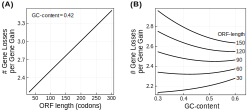
\includegraphics[scale=0.5]{Figures/Supp_figures/geneGainLossComplete2_new.pdf}
\caption{Genes are more likely to be independently lost twice, than being born once. The vertical axis in both panels shows the number of independent gene loss events that can occur relative to one gene gain event -- $\log(P_\textit{gene-gain})/\log(P_\textit{gene-loss})$. The horizontal axis shows the number of codons in the ORF \textbf{(A)}, and the GC-content \textbf{(B)}.}
\end{figure}

\subsection{Transcription first or ORF first}

\begin{figure}[H]
\centering
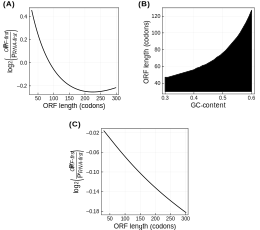
\includegraphics[scale=0.5]{Figures/Supp_figures/whichfirstComplete2_new.pdf}
\caption{Proto-genes with ORFs longer than 59 codons, emerge RNA-first, whereas proto-gens with shorter ORFs emerge ORF-first. The vertical axis shows the $\log_2$ transformed ratio of the probabilities of the ORF-first and the RNA-first trajectories, described as \textbf{(A)} a single-step process and \textbf{(C)} a two-step process. A negative value suggests that RNA-first trajectory is more likely than ORF-first trajectory, and \textit{vice versa}. In both panels, the horizontal axis denotes the number of codons in the ORF. \textbf{(B)} Filled area denotes the ORF length in codons (vertical axis) and the GC-content values (horizontal axis) at which ORF-first trajectory is more likely than RNA-first trajectory.}
\end{figure}

\subsection{ORF loss versus transcription loss}

\begin{figure}[H]
\centering
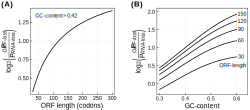
\includegraphics[scale=0.5]{Figures/Supp_figures/pLossComplete2_new.pdf}
\caption{ORF loss in proto-genes is more probable than transcription loss. The horizontal axis denotes the number of codons in the ORF \textbf{(A)} and GC-content \textbf{(B)}. The vertical axis shows the $\log_2$ transformed ratio of ORF loss and RNA loss probabilities, such that a positive value means ORF loss is more probable than RNA loss, and \textit{vice versa}.}
\end{figure}


\clearpage

\section{Model without core promoters}


\subsection{Effect on GC content on the probability of gene gain and loss}

We analysed the effect of effect on GC content on the number independent gene losses per gene gain, in the promoterless model.

\begin{figure}[H]
\centering
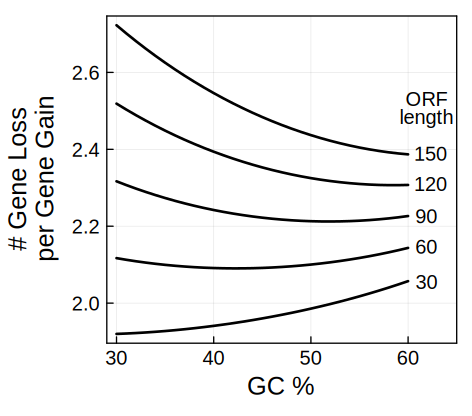
\includegraphics[scale=0.5]{Figures/Supp_figures/geneGainLoss_klengcr_promoterless.pdf}
\caption{Genes are more likely to be independently lost twice, than being born once. The vertical axis shows the number of independent gene loss events that can occur relative to one gene gain event -- $\log(P_\textit{gene-gain})/\log(P_\textit{gene-loss})$. The horizontal axis shows the GC-content.}
\end{figure}

\subsection{Exclusive ORF or transcription loss}

In the promoterless model, we made our analysis of gene loss more stringent by comparing the probabilities of two evolutionary scenarios, both of which begin with an intact proto-gene. In the first scenario, the ORF remains intact whereas the transcription is lost. The probability of this scenario ($P_\textit{onlyORF-loss}$) is described by: 

\vspace{-1ex}

\begin{equation}
P_\textit{onlyRNA-loss} = \frac{P_\textit{ORF-stay \vline\ RNA}}{P_\textit{ORF \vline \ RNA}} \times P_\textit{RNA-loss \vline\ ORF}
\end{equation}

We note that the probability that an ORF is not lost due to mutations ($P_\textit{ORF-stay \vline \ RNA}$), includes the probability that the ORF already exists ($P_\textit{ORF \vline \ RNA}$). To describe the conditional probability of ORF remaining undisrupted, given that it already exists, we divide $P_\textit{ORF-stay \vline \ RNA}$ by $P_\textit{ORF \vline \ RNA}$.

In the second scenario, transcription stays intact while ORF is lost. The probability of this scenario is: 

\vspace{-1em}
\begin{equation}
P_\textit{onlyORF-loss} = \frac{P_\textit{RNA-stay \vline\ ORF}}{P_\textit{RNA \vline \ ORF}} \times P_\textit{ORF-loss \vline\ RNA}
\end{equation}

We find that the second scenario (only ORF loss) is more plausible for all the analysed ORFs lengths.

\begin{figure}[H]
\centering
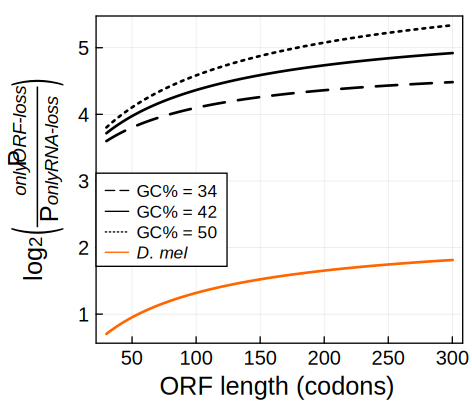
\includegraphics[scale=0.5]{Figures/Supp_figures/pLossOnly_promoterlessX.pdf}
\caption{Exclusive ORF loss in proto-genes is more probable than exclusive transcription loss. The vertical axis shows the $\log_2$ transformed ratio of only ORF loss and only RNA loss probabilities, such that a positive value means ORF loss is more probable than RNA loss, and \textit{vice versa}. The horizontal axis denotes the number of codons in the ORF. Black lines denote the probability values estimated from overall GC content (34\%, 42\% and 50\%) and the orange line denotes the probability values estimated from trimer and hexamer frequencies in \textit{D. melanogaster} intergenic genome.}
\end{figure}

\clearpage

\bibliographystyle{mybst}

\small
\bibliography{refs}

\end{document}
